\pdfminorversion=7
\documentclass[11pt,letterpaper]{article}

\usepackage[utf8]{inputenc}
\usepackage[T1]{fontenc}
\usepackage[french]{babel}
\frenchsetup{SmallCapsFigTabCaptions=false}
\usepackage{lmodern}
\usepackage{geometry}
\usepackage{graphicx}
\usepackage{grffile}
\usepackage{float}
\usepackage{booktabs}
\usepackage{longtable}
\usepackage{array}
\usepackage{tabularx}
\usepackage[table]{xcolor}
\usepackage{tikz}
\usepackage{eso-pic}
\usepackage{fancyhdr}
\usepackage{titlesec}
\usepackage[font=small,labelfont=bf]{caption}
\usepackage{microtype}
\usepackage{enumitem}
\usepackage{hyperref}

% Les ressources externes du rapport restent dans ces deux dossiers.
\graphicspath{{assets/}{img/}}

\geometry{
    letterpaper,
    left=0.95in,
    right=0.95in,
    top=1.55in,
    bottom=0.78in,
    headheight=18pt,
    headsep=18pt,
    footskip=28pt
}

\definecolor{tameoBlue}{HTML}{173B5C}
\definecolor{tameoLink}{HTML}{3A6B78}
\definecolor{tameoText}{HTML}{13283A}
\definecolor{tablerow}{RGB}{242, 244, 244}
\newcommand{\tameoCoverIndent}{0.20in}

% ---------------------------------------------------------------------------
% Informations du document
% ---------------------------------------------------------------------------
\newcommand{\tameoTitle}{Bateau IA - Groupe 25}
\newcommand{\tameoDocumentType}{Rapport Final de Description du Projet}
\newcommand{\tameoPdfTitle}{Bateau IA - Groupe 25 - Rapport Final de Description du Projet}
\newcommand{\tameoPdfAuthor}{Vinicius CAVALLARO, Loup COUERRE, Julia DIAS LEITE, Benoît MARCHÉ, Lucas DA SILVEIRA, Lucca DE SOUZA AMODIO, Maeva NOUKOUA, Javier TARAZONA}

\hypersetup{
    colorlinks=true,
    linkcolor=tameoBlue,
    urlcolor=tameoLink,
    pdftitle={\tameoPdfTitle},
    pdfauthor={\tameoPdfAuthor}
}

\setlength{\parindent}{0pt}
\setlength{\parskip}{0.55em}
\renewcommand{\arraystretch}{1.18}
\setlist[itemize]{label=-, leftmargin=*}
\newcolumntype{L}[1]{>{\raggedright\arraybackslash}p{#1}}
\newcolumntype{Y}{>{\raggedright\arraybackslash}X}
\setlength{\emergencystretch}{1.5em}

\titleformat{\section}
  {\sffamily\bfseries\LARGE\color{tameoBlue}}
  {\thesection}{0.75em}{}
\titleformat{\subsection}
  {\sffamily\bfseries\large\color{tameoBlue}}
  {\thesubsection}{0.75em}{}
\titleformat{\subsubsection}
  {\sffamily\bfseries\normalsize\color{tameoBlue}}
  {\thesubsubsection}{0.75em}{}
\titlespacing*{\section}{0pt}{1.3em}{0.65em}
\titlespacing*{\subsection}{0pt}{1.05em}{0.35em}
\titlespacing*{\subsubsection}{0pt}{0.85em}{0.25em}

\pagestyle{fancy}
\fancyhf{}
\renewcommand{\headrulewidth}{0pt}
\fancyfoot[R]{\thepage}

\newcommand{\tameoBranding}{%
    \begin{tikzpicture}[remember picture,overlay]
        \node[anchor=north east] at ([xshift=-1.16in,yshift=-0.58in]current page.north east)
            {
\includegraphics[width=1.98in]{tameo-logo.png}};
        \node[anchor=north east] at ([xshift=-1.18in,yshift=-1.12in]current page.north east)
            {
\includegraphics[width=2.05in,height=0.026in]{tameo-bar.png}};
    \end{tikzpicture}%
}

\newcommand{\tameoPersonCell}[1]{%
    \begin{minipage}[t]{2.6in}
        \raggedright
        \hyphenpenalty=10000
        \exhyphenpenalty=10000
        {\rmfamily\fontsize{10.8}{12.6}\selectfont #1\par}
    \end{minipage}%
}

\newcommand{\tameoAuthorsBlockA}{%
    \tameoPersonCell{Vinicius CAVALLARO}
    & \tameoPersonCell{Loup COUERRE}
    \tabularnewline[0.22in]
    \tameoPersonCell{Julia DIAS LEITE}
    & \tameoPersonCell{Benoît MARCHÉ}
}

\newcommand{\tameoAuthorsBlockB}{%
    \tameoPersonCell{Lucas DA SILVEIRA}
    & \tameoPersonCell{Lucca DE SOUZA AMODIO}
    \tabularnewline[0.22in]
    \tameoPersonCell{Maeva NOUKOUA}
    & \tameoPersonCell{Javier TARAZONA}
}

\newcommand{\maketameotitle}{%
    \begin{titlepage}
        \thispagestyle{empty}
        \begin{tikzpicture}[remember picture,overlay]
            \node[anchor=north east] at ([xshift=-1.37in,yshift=-2.42in]current page.north east)
                {
\includegraphics[width=1.82in]{tameo-logo.png}};
            \node[anchor=north west] at ([xshift=1.16in,yshift=-3.00in]current page.north west)
                {
\includegraphics[width=6.55in,height=0.115in]{tameo-bar.png}};
            \node[anchor=south east] at ([xshift=-1.16in,yshift=0.42in]current page.south east)
                {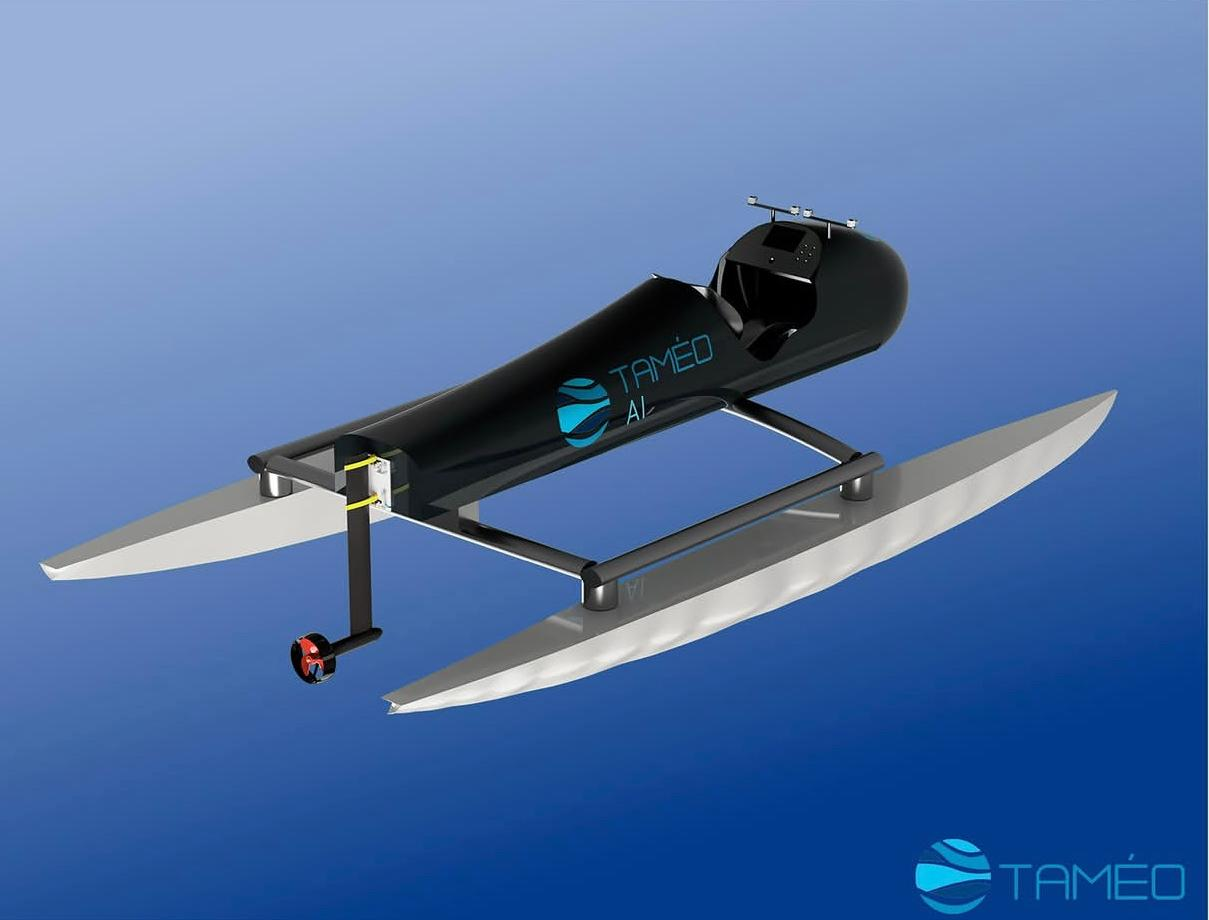
\includegraphics[width=3.1in]{image.png}};
        \end{tikzpicture}

        \vspace*{1.82in}
        {\hspace*{\tameoCoverIndent}\sffamily\bfseries\fontsize{42}{50}\selectfont\color{tameoBlue}\tameoTitle\par}
        \vspace{0.34in}
        {\hspace*{\tameoCoverIndent}\sffamily\itshape\fontsize{16}{20}\selectfont\color{tameoText}\tameoDocumentType\par}

        \vspace{0.34in}
        {\hspace*{\tameoCoverIndent}\sffamily\bfseries\fontsize{12}{14}\selectfont\color{tameoBlue}Auteurs:\par}
        \vspace{0.13in}
        \noindent\hspace*{\tameoCoverIndent}\makebox[0pt][l]{%
            \begin{tabular*}{5.95in}{@{\extracolsep{\fill}}ll@{}}
                \tameoAuthorsBlockA
            \end{tabular*}%
        }\par
        \vspace{0.18in}
        \noindent\hspace*{\tameoCoverIndent}\makebox[0pt][l]{%
            \begin{tabular*}{5.95in}{@{\extracolsep{\fill}}ll@{}}
                \tameoAuthorsBlockB
            \end{tabular*}%
        }

        \vspace{0.26in}
        \noindent\hspace*{\tameoCoverIndent}%
        \begin{minipage}{5.95in}
            {\sffamily\bfseries\fontsize{12}{14}\selectfont\color{tameoBlue}Encadrants:\par}
            \vspace{0.08in}
            {\rmfamily\fontsize{10.8}{13}\selectfont M. TARUFFI \quad M. XERRI \quad M. FAUL\par}
            \vspace{0.18in}
            {\sffamily\fontsize{10.8}{13}\selectfont\color{tameoText}Projet d'Ingénierie en Équipe (PIE) 2025-2026\par}
            {\sffamily\fontsize{10.8}{13}\selectfont\color{tameoText}Monaco Energy Boat Challenge 2026\par}
            {\sffamily\fontsize{10.8}{13}\selectfont\color{tameoText}Avril 2026\par}
        \end{minipage}

        \vfill
    \end{titlepage}
}

\makeatletter
\newcommand{\styledtableofcontents}{%
    \thispagestyle{fancy}
    \vspace*{1.05in}
    {\sffamily\bfseries\fontsize{24}{29}\selectfont\color{tameoBlue}Table des matières\par}
    \vspace{0.85in}
    \begingroup
    \parskip=0.18em
    \@starttoc{toc}
    \endgroup
    \newpage
}
\makeatother

\begin{document}

\maketameotitle
\setcounter{page}{2}
\AddToShipoutPictureBG{\tameoBranding}
\styledtableofcontents

\section{Introduction}
Ce rapport final de gestion de projet a pour objectif de synthétiser l'intégralité du travail accompli par l'équipe Bateau IA - 26 dans le cadre du Projet d'Ingénierie en Équipe (PIE) de l'ENSTA Paris. Il documente la transition entre la phase de conception initiale et la réalisation finale d'un prototype de navigation autonome destiné au Monaco Energy Boat Challenge (MEBC) 2026. Ce document sert à la fois de bilan technique pour nos encadrants et de base de connaissances pour la passation aux promotions futures, tout en analysant les écarts entre nos prévisions et les résultats obtenus.

\subsection{Enjeux, besoins et périmètre du projet}
L'ENSTA Paris, forte de ses succès passés en classe "Energy", a décidé cette année de relever un nouveau défi technique en participant pour la première fois à la classe IA du MEBC. Cette compétition internationale, organisée par le Yacht Club de Monaco, constitue un incubateur de recherche pour le yachting durable et innovant.

Le besoin fondamental de notre projet est de développer un système autonome (AMS) capable de piloter un bateau sans aucune intervention humaine. Les enjeux majeurs se déclinent en trois axes :
\begin{itemize}
    \item \textbf{Conformité et sécurité :} Satisfaire aux inspections techniques onshore et aux "water tests", tout en garantissant une supervision sécurisée (kill cord, procédures de reset physique) et une absence totale de contrôle à distance.
    \item \textbf{Performance opérationnelle :} Assurer une navigation précise et robuste face aux perturbations marines (vagues, reflets) lors des épreuves de Sprint, de Slalom et de Docking.
    \item \textbf{Pédagogique et associatif :} Valoriser l'expertise de l'ENSTA Paris et de l'association TAMÉO à travers une solution d'ingénierie complète intégrant mécanique, électronique et intelligence artificielle.
\end{itemize}

Le périmètre de notre intervention s'est concentré sur la création et l'intégration du programme d'IA, subdivisé en trois pôles : la Détection et Vision (reconnaissance d'obstacles), la Trajectoire et Navigation (inférence de la route optimale) et les Tests et Intégration (conversion en commandes exécutables).

\subsection{Rappel des objectifs et évolutions}
Nos objectifs initiaux étaient de construire une architecture AS complète permettant de percevoir, décider et contrôler le véhicule de manière totalement autonome. Au fil du projet, ces objectifs ont été affinés pour adopter une stratégie \textbf{MVP (Minimum Viable Product)} afin de garantir la fiabilité du système avant la performance pure :
\begin{itemize}
    \item \textbf{Perception :} Détecter et suivre les bouées (fixes et mobiles) via un modelo de type YOLO, en produisant des sorties exploitables (bounding boxes, indices de confiance) pour le pilotage.
    \item \textbf{Localisation et Décision :} Assurer une localisation robuste (GPS/RTK) et construire une logique de mission par épreuve, notamment la figure en 8 et l'approche lente de "Docking" sans contact avec le quai.
    \item \textbf{Sûreté :} Implémenter une télémétrie de sécurité vers la terre et un mode "Failsafe" garantissant l'arrêt immédiat de la propulsion en cas de situation critique.
\end{itemize}

\textbf{Évolution notable :} Par rapport au rapport initial, le périmètre a été rationalisé pour privilégier un mode de navigation "conservateur" (vitesse réduite et évitement grossier) lors des épreuves complexes comme le Slalom avec bouée dynamique, afin de minimiser les risques de collision frontale et de disqualification.

\subsection{Parties Prenantes}
L'écosystème du projet implique plusieurs acteurs clés :
\begin{itemize}
    \item \textbf{TAMÉO :} Client final, exploitant et association porteuse du projet.
    \item \textbf{ENSTA Paris :} Tutelle pédagogique et source de financement.
    \item \textbf{MEBC :} Comité organisateur imposant le règlement technique et de sécurité.
    \item \textbf{Sponsors (DGA, SaveMyBattery) :} Fournisseurs de composants et support technique.
\end{itemize}

\section{Rappel de l’organisation de l’équipe et matrice RACI}
\subsection{Organisation structurelle et répartition fonctionnelle}
L'équipe est structurée pour assurer une synergie entre la conception matérielle et l'IA, sous la direction technique globale de Loup Couerre. Afin de répondre aux exigences de clarté sur les missions de chacun, les rôles sont définis comme suit :

\subsubsection{Pôle Conception du Bateau (Dirigé par Henri Cressot)}
Ce bloc assure la viabilité physique et logicielle de bas niveau de l'AMS.
Dirigé par Henri Cressot, ce bloc assure la base matérielle et logicielle bas niveau nécessaire au fonctionnement de l'IA

\begin{itemize}
    \item \textbf{Structure et Châssis (Clément Gilbert, Mathieu Oudard, Romain Guinjard, Paul Arakelian, Nolann Laurent) :} Responsables du design mécanique, de l'étanchéité du cockpit et de l'intégration rigide des supports de capteurs (ZED et GPS) pour éviter les vibrations parasites.
    \item \textbf{Direction et Propulsion (Aurélien Lebrat, Martin Ménard, Armand Rodrik, Mayeul Baltzinger, Victor Sevel) :} En charge du dimensionnement des servomoteurs, de la calibration de la poussée des moteurs électriques et de la cinématique de direction.
    \item \textbf{Électronique (Taha Assebbane, Simon Lefranc, Léo Paille, Arno Askenazy) :} Développement du système de distribution de puissance, intégration des batteries sécurisées et mise en place des circuits physiques d'arrêt d'urgence (E-Stop).
    \item \textbf{Informatique embarquée (Julia Dias, Maeva Noukoua, Benoît Marche, Séverin Vaillant, Thomas Pelleschi, Léonard Fraticelli) :} Développement des drivers ROS pour les capteurs et gestion du middleware de communication (Bus CAN) entre le calculateur IA et les actionneurs.
\end{itemize}

\subsubsection{Pôle Intelligence Artificielle (Co-dirigé par E. Le Hay et J. Tarazona)}
Ce bloc constitue le cœur algorithmique du système autonome.
\begin{itemize}
    \item \textbf{Détection et Vision (Ewen Le Hay, Javier Tarazona, Lucas Absalao, Florian Verne) :} Responsables de l'entraînement du modèle YOLO, de la constitution du dataset marin et de l'optimisation de l'inférence temps réel sur le GPU embarqué.
    \item \textbf{Trajectoire et Navigation (Lucca Amodio, Vinicius Zancheta, Julien Ye, Yuheng Zhang) :} Développement de la logique de mission (Machine à états), des algorithmes de planification de route par waypoints et des règles d'évitement d'obstacles.
    \item \textbf{Tests et Intégration (Thomas Wawrzyniak, Clément Pieutchot, Enzo Sawaya) :} Pivot central assurant la liaison entre les pôles. Ils valident la boucle de contrôle complète et s'assurent de la fiabilité des failsafes logiciels avant les tests sur l'eau.
\end{itemize}

\subsection{Évolution de la Matrice RACI}

\subsubsection{Matrice Initiale (Silos de conception)}
Au début du projet, les rôles étaient isolés par domaine d'expertise, ce qui a causé des difficultés lors de l'intégration des drivers avec les modèles d'IA.
\begin{center}
\small
\begin{tabularx}{\textwidth}{lXXXX}
\toprule
\textbf{Tâche / Rôle} & Vision & Navigation & Intégration & Direction \\
\midrule
Entraînement Modèle & R/A & I & I & - \\
Path Planning & C & R/A & I & - \\
Câblage Physique & - & - & R/A & C \\
\bottomrule
\end{tabularx}
\end{center}

\subsubsection{Matrice Finale (Approche Intégrée)}
La nouvelle matrice introduit une transversalité nécessaire pour maîtriser les latences et garantir la sûreté de l'AMS.
\rowcolors{2}{tablerow}{white}
\begin{center}
\small
\begin{tabularx}{\textwidth}{lXXXXX}
\toprule
\textbf{Tâche Globale} & \textbf{Vision} & \textbf{Nav.} & \textbf{Intég.} & \textbf{Elec.} & \textbf{Dir. Tech.} \\
\midrule
Validation Perception & R/A & C & C & I & I \\
Logique Mission (MVP) & I & R & A & I & C \\
Middleware CAN/ROS & C & I & R/A & C & I \\
Tests de Sûreté & I & I & R & I & A \\
Gestion de Configuration & C & C & R/A & I & I \\
\bottomrule
\end{tabularx}
\end{center}

\medskip
\textit{Analyse de la transition RACI :} L'analyse comparative montre un changement de paradigme. La première matrice souffrait d'un manque de définition sur l'intégration système. Dans la version actualisée, le pôle « Tests et Intégration » est devenu le pivot central. L'introduction explicite de la gestion du middleware et de la configuration Git a permis de clarifier « qui fait quoi » lors des phases critiques. La sécurité est désormais une tâche partagée où l'Intégration réalise et la Direction Technique approuve, assurant une double validation.

\subsection{Remédiation organisationnelle}
Depuis le rapport initial, nous avons renforcé le pôle Informatique Embarquée pour servir de pont avec l'IA. La distinction entre « Perception » et « Navigation » a été durcie pour permettre un débogage modulaire plus efficace, évitant ainsi de confondre les erreurs de détection avec les erreurs de planification de route.


\section{Liste des livrables fournis}
L'ensemble des livrables a été conçu pour répondre aux exigences du MEBC.

\subsection{Livrables matériels (Hardware)}
\begin{itemize}
    \item \textbf{Plateforme Bateau IA :} Unité nautique fonctionnelle équipée de sa propulsion électronique.
    \item \textbf{Capteur de vision :} Caméra stéréo ZED pour la perception d'obstacles.
    \item \textbf{Système de localisation :} Antenne GPS compatible RTK.
    \item \textbf{Unité de calcul :} GPU embarqué haute performance pour l'IA temps réel.
    \item \textbf{Sécurité :} Kill cord, E-stop conforme et système de télémétrie 2 NM.
\end{itemize}

\subsection{Livrables logiciels (Software)}
\begin{itemize}
    \item \textbf{Module Perception :} Algorithme YOLO pour la détection de bouées.
    \item \textbf{Module Navigator :} Logique de mission gérant les séquences de waypoints.
    \item \textbf{Module Avoidance :} Règles d'évitement simples par zones de danger.
    \item \textbf{Interface :} Dashboard live affichant bounding boxes et télémétrie.
\end{itemize}

\subsection{Livrables documentaires}
\rowcolors{2}{tablerow}{white}
\begin{tabularx}{\textwidth}{lX}
\toprule
\textbf{Type de dossier} & \textbf{Contenu principal} \\
\midrule
Dossier de Conception & Cahier des charges, WBS, GANTT détaillé. \\
Dossier de Réalisation & Architecture finale, inventaire matériel, logs de tests. \\
Guide d'Exploitation & Manuel pilote et guide d'installation logicielle. \\
Analyse de Risque Finale & Matrice de criticité mise à jour avec mesures de mitigation. \\
Manuels Techniques & Manuel du module Vision et Manuel BlueBoat. \\
\bottomrule
\end{tabularx}

\section{Déroulement du projet et analyse thématique}

\subsection{Chronologie des jalons et événements majeurs}
Le cycle de vie du projet \textbf{Bateau IA - 26} a été rythmé par une série d'étapes critiques, allant de la théorie à la confrontation avec le milieu marin. Le projet a débuté en janvier 2026 par une phase de recherche intensive pour fixer l'architecture logicielle.

Dès le mois de février, l'équipe a dû finaliser les spécifications pour lancer les commandes lourdes, notamment la caméra ZED et l'unité de calcul GPU, afin d'anticiper les délais de livraison. Le mois de mars a marqué un tournant avec le début de la collecte de données sur le terrain, essentielle pour entraîner notre modèle de détection d'obstacles. En avril, nous avons fait face à notre premier incident majeur : une instabilité critique des drivers GPU sous Docker, ce qui a paralysé le développement pendant une semaine.

L'intégration sur le \textbf{BlueBoat} s'est réellement concrétisée en mai, ouvrant la voie à une phase de simulation 2D intensive pour combler l'écart de performance entre le virtuel et le réel. Enfin, le mois de juin a été dédié à la validation finale des procédures de sécurité et aux tests de mission complète avant le départ pour Monaco.

\subsection{Analyse thématique du projet}

\subsubsection{Pilotage et dynamique d'équipe}
La gestion de ce projet a révélé la difficulté de coordonner deux promotions (PIE et PIC) sur un objectif commun. Le pilotage a d'abord souffert d'un manque de visibilité sur les tâches quotidiennes, ce qui a confirmé le risque de « défaillance de communication » identifié dans notre analyse initiale. L'absence de jalons de démonstration intermédiaires a failli retarder l'intégration logicielle. Pour y remédier, nous avons instauré des séances de travail obligatoires au \textbf{FabLab} chaque jeudi, transformant un mode de fonctionnement asynchrone en une collaboration directe. Ce changement de méthode a permis de clarifier « qui fait quoi » et de stabiliser l'interface entre le pôle informatique et le pôle mécanique.

\subsubsection{Conception : du Reinforcement Learning au MVP}
Sur le plan de la conception, notre ambition initiale d'utiliser l'apprentissage par renforcement (RL) s'est heurtée à la réalité de la complexité embarquée. Les premiers tests ont montré que les décisions du RL étaient trop lourdes pour le calculateur et que les comportements induits pouvaient être dangereux pour l'intégrité du bateau. Cet échec nous a conduits à une décision stratégique forte : pivoter vers une architecture de type \textbf{Minimum Viable Product (MVP)}. Nous avons remplacé la planification complexe par une machine à états robuste (IDLE, RUN, SAFE) couplée à un évitement d'obstacles basé sur des zones de danger fixes dans l'image. Cette simplification a paradoxalement augmenté la fiabilité du système en réduisant l'incertitude décisionnelle.

\subsubsection{Réalisation et défis de l'informatique embarquée}
La phase de réalisation physique a mis en lumière des problèmes de bas niveau souvent sous-estimés en phase d'étude. L'interfaçage avec le bus CAN pour le contrôle de la direction et de la propulsion a généré des pertes de messages et des latences critiques. Ces bugs logiciels, couplés à une consommation électrique du hardware de calcul plus élevée que prévu, ont nécessité une optimisation drastique de notre middleware. Nous avons dû implémenter des garde-fous pour éviter que des commandes irréalistes ne soient envoyées aux actionneurs en cas de lag logiciel, garantissant ainsi que le bateau reste dans son enveloppe de sécurité opérationnelle.

\subsubsection{Validation et gestion des échecs de perception}
La campagne de tests finaux a été le juge de paix de notre système de vision. Nous avons constaté une limite technologique majeure : l'algorithme YOLO peinait à détecter les bouées à 60 mètres sous l'effet des reflets solaires, un risque environnemental que nous avions pourtant identifié. Plutôt que de chercher une solution logicielle miracle, nous avons intégré cette faiblesse dans notre logique de navigation. En cas de non-détection ou de doute statistique (faux négatifs), le système déclenche désormais un mode « conservateur » qui réduit la vitesse et maintient le cap actuel jusqu'à la levée de l'incertitude. Cette analyse constructive de nos échecs de perception nous a permis de livrer un système qui, s'il n'est pas infaillible, est intrinsèquement sûr pour la compétition.

\section{Mise à jour de la planification, des coûts et des risques}

\subsection{Planification réelle (Gantt actualisé)}
\begin{figure}[h]
    \centering
    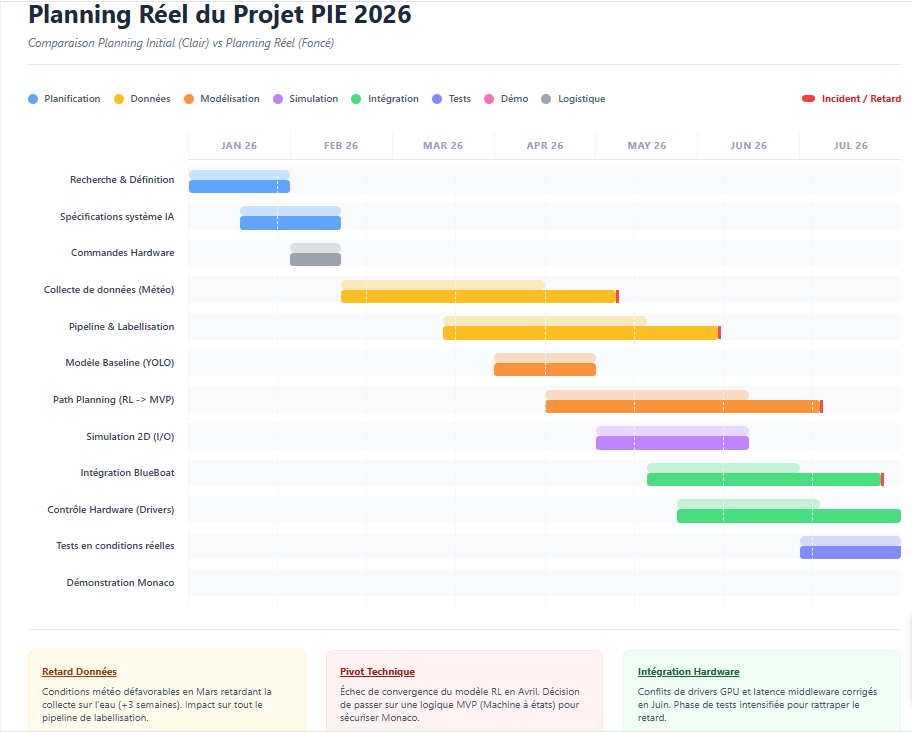
\includegraphics[width=0.7\linewidth]{Captura de tela 2026-04-10 141826.png}
    \caption{Évolution du planning initial vers le planning réel.}
    \label{fig:placeholder}
\end{figure}

\subsubsection{Analyse des écarts de planification}
L'analyse du GANTT réel met en lumière des décalages liés à la météo en mars (+3 semaines sur la collecte de données) et aux drivers GPU en avril. Le passage au MVP a toutefois permis de compresser la phase de modélisation pour rattraper le retard sur l'intégration BlueBoat.

\subsection{Bilan des coûts (Budget actualisé)}
Le budget a été maintenu à 50 481,13 €.

\rowcolors{2}{tablerow}{white}
\begin{tabularx}{\textwidth}{lrX}
\toprule
\textbf{Poste de dépense} & \textbf{Montant (€)} & \textbf{Description} \\
\midrule
Technique Bateau IA & 15 000,00 € & Capteurs (ZED, GPS RTK), calculateurs haute performance. \\
Technique Bateau EC & 10 000,00 € & Maintenance et composants partagés avec la classe Energy. \\
Blue Boat & 7 000,00 € & Plateforme de test et flotteurs. \\
MEBC 2026 & 7 000,00 € & Frais d'inscription, logistique et transport vers Monaco. \\
Fond de roulement & 7 881,13 € & Réserve pour imprévus techniques et consommables. \\
Communication \& Divers & 3 600,00 € & Permis, frais bancaires, supports de communication. \\
\bottomrule
\end{tabularx}

\subsection{Évolution et gestion des risques}
Les risques les plus critiques identifiés (Latence Vision, Collision) ont été mitigés par le pivot MVP et l'optimisation middleware. Le risque environnemental (reflets) reste géré par un comportement dégradé du bateau (vitesse réduite).

\section{Proposition d'une organisation de remédiation}
Une analyse rétrospective du projet suggère l'adoption d'une stratégie de développement dite « Dual-Track » pour les itérations futures. L'une des difficultés majeures rencontrées fut le pivot tardif du modèle de Reinforcement Learning vers une logique MVP, causé par un manque de convergence algorithmique. Pour y remédier, il serait pertinent de maintenir deux pistes de développement parallèles dès le premier mois : une piste de base déterministe par waypoints, assurant un système fonctionnel en permanence, et une piste de recherche avancée pour l'innovation, évitant ainsi de mettre en péril la participation à la compétition en cas de blocage technologique.

Sur le plan technique, l'intégration précoce via un banc de test « Hardware-in-the-Loop » (HIL) est indispensable. Cette année, les problèmes de drivers GPU et les latences du middleware n'ont été identifiés qu'en phase d'intégration physique tardive sur le BlueBoat. En concevant un banc de test électronique complet dès la réception des premiers composants, l'équipe pourrait identifier les goulots d'étranglement de données et les incompatibilités logicielles bien avant la mise à l'eau, sécurisant ainsi la phase critique de validation finale.

En ce qui concerne la gestion de l'environnement, l'utilisation d'une simulation 3D haute fidélité (type Gazebo ou Unity) incluant des shaders réalistes de reflets marins permettrait de s'affranchir des aléas météorologiques. Les retards de collecte de données en mars ont montré qu'une dépendance stricte aux tests réels est un risque temporel fort. Simuler des conditions marines variées permettrait d'entraîner et de tester les modèles de perception (YOLO) de manière continue, indépendamment des conditions extérieures à Palaiseau.

Enfin, la gouvernance de l'équipe gagnerait à utiliser des outils de gestion de tâches dynamiques tels que Kanban ou Trello pour briser les silos d'information entre les pôles PIE et PIC. La communication hebdomadaire s'est parfois révélée insuffisante pour suivre l'avancement granulaire des tâches. Une traçabilité numérique systématique, couplée à des « sprints » de deux semaines, assurerait une transparence totale sur les points de blocage et faciliterait la passation d'informations techniques cruciales, évitant les redondances constatées lors de cette édition.

\section{Conclusion}
En conclusion, ce projet d'ingénierie a permis de poser les fondations essentielles de la participation de l'ENSTA Paris à la classe IA du Monaco Energy Boat Challenge 2026. Bien que le système ne soit pas encore intégralement opérationnel à ce stade du calendrier, l'équipe a réussi à établir une architecture logicielle cohérente et à valider les premiers modules critiques de perception et de localisation. Le passage d'une ambition technologique initiale très complexe vers une stratégie de type Minimum Viable Product (MVP) a été une étape déterminante pour recentrer nos efforts sur la fiabilité des fonctions de base et la sûreté du véhicule en milieu marin.

Sur le plan de la gestion, le projet a constitué un véritable laboratoire d'apprentissage face à l'imprévu. Nous avons dû composer avec des défis d'intégration logicielle majeurs, notamment les instabilités de drivers et les latences du bus de données, tout en respectant un budget conséquent de 50 481,13 €. La coordination entre les huit membres de l'équipe et les différentes parties prenantes a exigé une grande adaptabilité, nous forçant à transformer chaque difficulté technique en une opportunité de simplification et de sécurisation du système autonome.

Enfin, si le prototype nécessite encore des phases de tests intensives avant d'être totalement prêt pour les épreuves de juillet à Monaco, le travail de documentation réalisé assure une continuité solide pour la phase finale du challenge. Les dossiers de conception et les manuels d'exploitation fournis constituent un héritage précieux pour les étudiants de première année qui poursuivront le développement et porteront les couleurs de TAMÉO. Nous clôturons ce mandat avec la satisfaction d'avoir défriché un terrain technologique inédit pour l'école et d'avoir livré une plateforme de base résiliente et prometteuse pour l'avenir de la classe IA.


\end{document}
